\documentclass[aspectratio=169,10pt]{beamer}
\usepackage{booktabs,tabularx,graphicx,array}
\usetheme{default}
\usecolortheme{seahorse}
\setbeamertemplate{navigation symbols}{}
\setbeamertemplate{footline}{\hfill\scriptsize\insertframenumber/\inserttotalframenumber\hspace{2mm}\vspace{1mm}}
\setbeamerfont{frametitle}{size=\normalsize}
\graphicspath{{plots/}}
\definecolor{part}{RGB}{200,120,0}\definecolor{bad}{RGB}{180,30,30}\definecolor{set}{RGB}{90,90,90}\definecolor{new}{RGB}{40,80,160}\definecolor{ok}{RGB}{30,120,60}
\newcommand{\RAN}{\textcolor{part}{\textbf{Ran, not validated}}}
\newcommand{\PART}{\textcolor{bad}{\textbf{Ran, did not finish}}}
\newcommand{\SETUP}{\textcolor{set}{\textbf{Setup only}}}
\newcommand{\PLAN}{\textcolor{new}{\textbf{Planned, not started}}}
\newcommand{\VYES}{\textcolor{ok}{\textbf{data in hand}}}
\newcommand{\VDL}{\textcolor{part}{\textbf{public, to download}}}
\newcommand{\VNO}{\textcolor{bad}{\textbf{not available}}}
\newcolumntype{L}[1]{>{\raggedright\arraybackslash}p{#1}}
\newcolumntype{Y}{>{\raggedright\arraybackslash}X}
% one row of the case table
\newcommand{\rw}[2]{\textbf{#1} & #2\\[0.6pt]}
% case table: #1 width
\newenvironment{casetab}[1]{\fontsize{7.4}{8.7}\selectfont\setlength{\tabcolsep}{3pt}\renewcommand{\arraystretch}{1.05}\tabularx{#1}{@{}L{2.25cm}Y@{}}\toprule}{\bottomrule\endtabularx}
\newcommand{\status}[2]{\vspace{-1mm}{\footnotesize Status: #1 \hfill #2}\par\vspace{0.6mm}}

\title{Planned Turbomachinery Cases: Not Yet Validated}
\subtitle{Geometry, physics, boundary conditions, rotation model and validation data for each case}
\author{OpenFOAM v2412 turbomachinery programme}
\date{5 October 2026}
\begin{document}
\begin{frame}\titlepage\end{frame}

\begin{frame}{Scope and how to read each slide}
\small
\begin{itemize}
\item 19 cases: every planned case not yet compared with experiment. The 4 validated cases (ERCOFTAC pump, FDA blood pump, PPTC open water, single-channel pump) are not repeated.
\item One slide per case, same rows on every slide: geometry, domain and mesh, fluid, physics and solver, rotation model, boundary conditions, operating point, validation data, references, status.
\item Rig facts (geometry, operating point, data) were checked on 5 Oct 2026 against the primary sources listed on each slide and in the reference list at the end. Set-up values for built cases come from the case dictionaries and logs. Set-ups not yet built are marked \emph{planned}: they are proposals, not facts.
\end{itemize}
\vspace{1mm}
\scriptsize
\begin{tabular}{@{}ll@{\hspace{3mm}}ll@{}}\toprule
\multicolumn{2}{@{}l}{\textbf{Status}} & \multicolumn{2}{l}{\textbf{Validation data}}\\\midrule
\RAN & solver ran, no comparison yet & \VYES & on this machine\\
\PART & solver crashed or did not converge & \VDL & open, to download\\
\SETUP & dictionaries only, no mesh or run & \VNO & not public or none\\
\PLAN & in the plan, nothing built & & \\\bottomrule
\end{tabular}
\end{frame}

\begin{frame}{Overview of the 19 cases}
\vspace{-2mm}\fontsize{6.3}{7.3}\selectfont\renewcommand{\arraystretch}{0.95}\setlength{\tabcolsep}{3pt}
\begin{tabularx}{\textwidth}{@{}r L{2.6cm} L{2.4cm} L{2.4cm} L{3.0cm} Y@{}}\toprule
\# & Case & Machine & Physics & Rotation model & Validation data\\\midrule
1 & Francis-99 & Francis turbine & incompr. RANS & MRF + mixingPlane & \VYES\\
2 & NREL Phase VI & HAWT wind turbine & incompr. RANS & MRF & \VDL\\
3 & VKI LS89 & transonic turbine vane & compressible & none (cascade) & \VYES\\
4 & NASA Rotor 37 & transonic compressor & compressible & MRF & \VYES\\
5 & Timisoara swirl generator & swirl gen. / runner & incompr. URANS & sliding mesh (AMI) & \VDL\ (paper)\\
6 & axialTurbine (6 variants) & axial hydro stage & incompr. RANS/URANS & SRF, MRF, mixingPlane, AMI & \VNO\ (no experiment)\\
7 & Turbine-99 & Kaplan draft tube & incompr. RANS & none (rotating cone wall) & \VNO\ (raw data offline)\\
8 & Aachen 1.5-stage & axial gas turbine & compressible & MRF + mixingPlane & \VNO\ (SU2 result only)\\
9 & Pelton (NTNU) & impulse turbine & VOF two-phase & sliding mesh (ACMI) & efficiency only, CAD on request\\
10 & Mini-ORC (TU Delft) & radial-inflow turbine & real-gas compressible & MRF + mixingPlane & \VNO\ (no measurements)\\
11 & PPTC cavitating & propeller & cavitation (VOF) & MRF or sliding mesh & \VYES\\
12 & SHF impeller & centrifugal pump (air model) & incompr. RANS & MRF or frozen rotor & published (PIV, wall pressure)\\
13 & NASA Stage 35 & axial compressor stage & compressible & MRF + mixingPlane & \VDL\\
14 & Radiver & centrifugal compressor & compressible & MRF + mixingPlane & \VDL\\
15 & Krain impeller & centrifugal compressor & compressible & MRF & published, geometry incomplete\\
16 & NASA HECC & centrifugal compressor & compressible & MRF + mixingPlane & \VDL\\
17 & NASA SDT R4 & turbofan fan & compressible & MRF + mixingPlane & data public, CAD not\\
18 & MEXICO rotor & HAWT wind turbine & incompr. RANS & MRF & consortium access\\
19 & Wells turbine / OWC & wave-energy air turbine & oscill. flow, VOF chamber & sliding mesh or MRF & per chosen rig\\\bottomrule
\end{tabularx}
\end{frame}

%================ A. Ran, not validated
\section{Ran, not validated}

\begin{frame}{1. Francis-99 (NTNU model Francis turbine, 2nd workshop)}
\status{\PART: 1000 iterations, residuals $\sim10^{-2}$; serial only}{Validation data: \VYES}
\begin{casetab}{\textwidth}
\rw{Geometry}{NTNU Waterpower Lab model: 1:5.1 model of the Tokke prototype: spiral casing, 14 stay vanes, 28 guide vanes, runner 15 blades + 15 splitters, draft tube. Mesh used: guide-vane angle 6.72$^\circ$}
\rw{Domain and mesh}{Single passage of guide vane and runner (periodic) + full draft tube; workshop mesh 1.89M cells, 141 patches; non-orth.\ 72.6$^\circ$, skewness 3.94}
\rw{Fluid}{Water, incompressible, Newtonian}
\rw{Physics and solver}{Steady RANS, \texttt{simpleFoam}, standard $k$-$\varepsilon$; PBiCGStab for $p$, relaxation 0.1, upwind U}
\rw{Rotation model}{\textbf{MRF} runner, case value $\omega=-35.123$ rad/s (335.4 rpm; measured at PL: 34.87 rad/s); \textbf{mixingPlane} at GV--runner and runner--draft tube; 8 periodic \texttt{ggi} pairs (TurboWG libraries)}
\rw{Boundary conditions}{Inlet (GV inflow): prescribed velocity, radial $-1.428$, tangential $-2.14$ m/s, axial 0; outlet: static pressure; walls: no-slip with wall functions}
\rw{Operating point}{\textbf{Part load}: workshop data give $\alpha=6.72^\circ$ for PL (BEP 9.84$^\circ$, HL 12.46$^\circ$); PL $H\approx11.87$ m, $Q\approx0.14$ m$^3$/s}
\rw{Validation data}{NTNU 2nd-workshop data, downloaded: steady pressure at VL2 (vaneless space), DT5, DT6 (draft tube); steady velocity; PIV on 3 draft-tube lines (\texttt{f99w2-exp-*})}
\rw{References}{Trivedi, Cervantes, Gandhi, Dahlhaug (2013) \emph{J.\ Fluids Eng.}\ 135(11):111102; Francis-99 2nd workshop data (NTNU, Dec 2016)}
\rw{Gap / next step}{Continue to convergence ($\varepsilon$ and mixingPlane flux still oscillate), set $\omega$ to the PL value, then compare pressure and PIV}
\end{casetab}
\end{frame}

\begin{frame}{2. NREL Phase VI (Unsteady Aerodynamics Experiment, wind turbine)}
\status{\RAN: 7 wind speeds, 2000 iterations each}{Validation data: \VDL}
\begin{columns}[T]
\column{.70\textwidth}
\begin{casetab}{\linewidth}
\rw{Geometry}{2-bladed stall-regulated HAWT, S809 airfoil, $D=10.058$ m, tip pitch 3$^\circ$, NASA Ames 24.4$\times$36.6 m tunnel; lofted in Python from the chord/twist tables of TP-500-29955 (root transition, rounded tip cap)}
\rw{Domain and mesh}{Full rotor in a box; STL $\to$ \texttt{snappyHexMesh}, 1.31M cells; 1 checkMesh test failed (146 skewed faces, max 10.8)}
\rw{Fluid}{Air, incompressible, $\nu=1.5\times10^{-5}$ m$^2$/s}
\rw{Physics and solver}{Steady RANS, \texttt{simpleFoam}, $k$-$\omega$ SST, TI 1\% (assumed)}
\rw{Rotation model}{\textbf{MRF} rotor zone, $\omega=7.54$ rad/s (72 rpm)}
\rw{Boundary conditions}{Inlet: fixed velocity 5--25 m/s; outlet: $p=0$, \texttt{inletOutlet} U; far field: slip; blades: no-slip}
\rw{Operating point}{Sequence S (upwind, rigid, 3$^\circ$ tip pitch, 5--25 m/s), 0$^\circ$ yaw subset; 72 rpm; $U_\infty$ = 5, 7, 10, 13, 15, 20, 25 m/s}
\rw{Validation data}{Shaft torque, root flap moment; $C_p$ from 22 taps at each of 30, 46.6, 63.3, 80, 95\% span, integrated to $C_n$, $C_t$; only TP-500-29955 is here, measured data (TP-500-29494, DOE Wind Data Hub) to download}
\rw{References}{Hand et al.\ (2001) NREL/TP-500-29955; Simms et al.\ (2001) NREL/TP-500-29494}
\rw{Gap / next step}{5 m/s torque has the wrong sign; fix mesh quality, then compare torque and $C_p$}
\end{casetab}
\column{.28\textwidth}
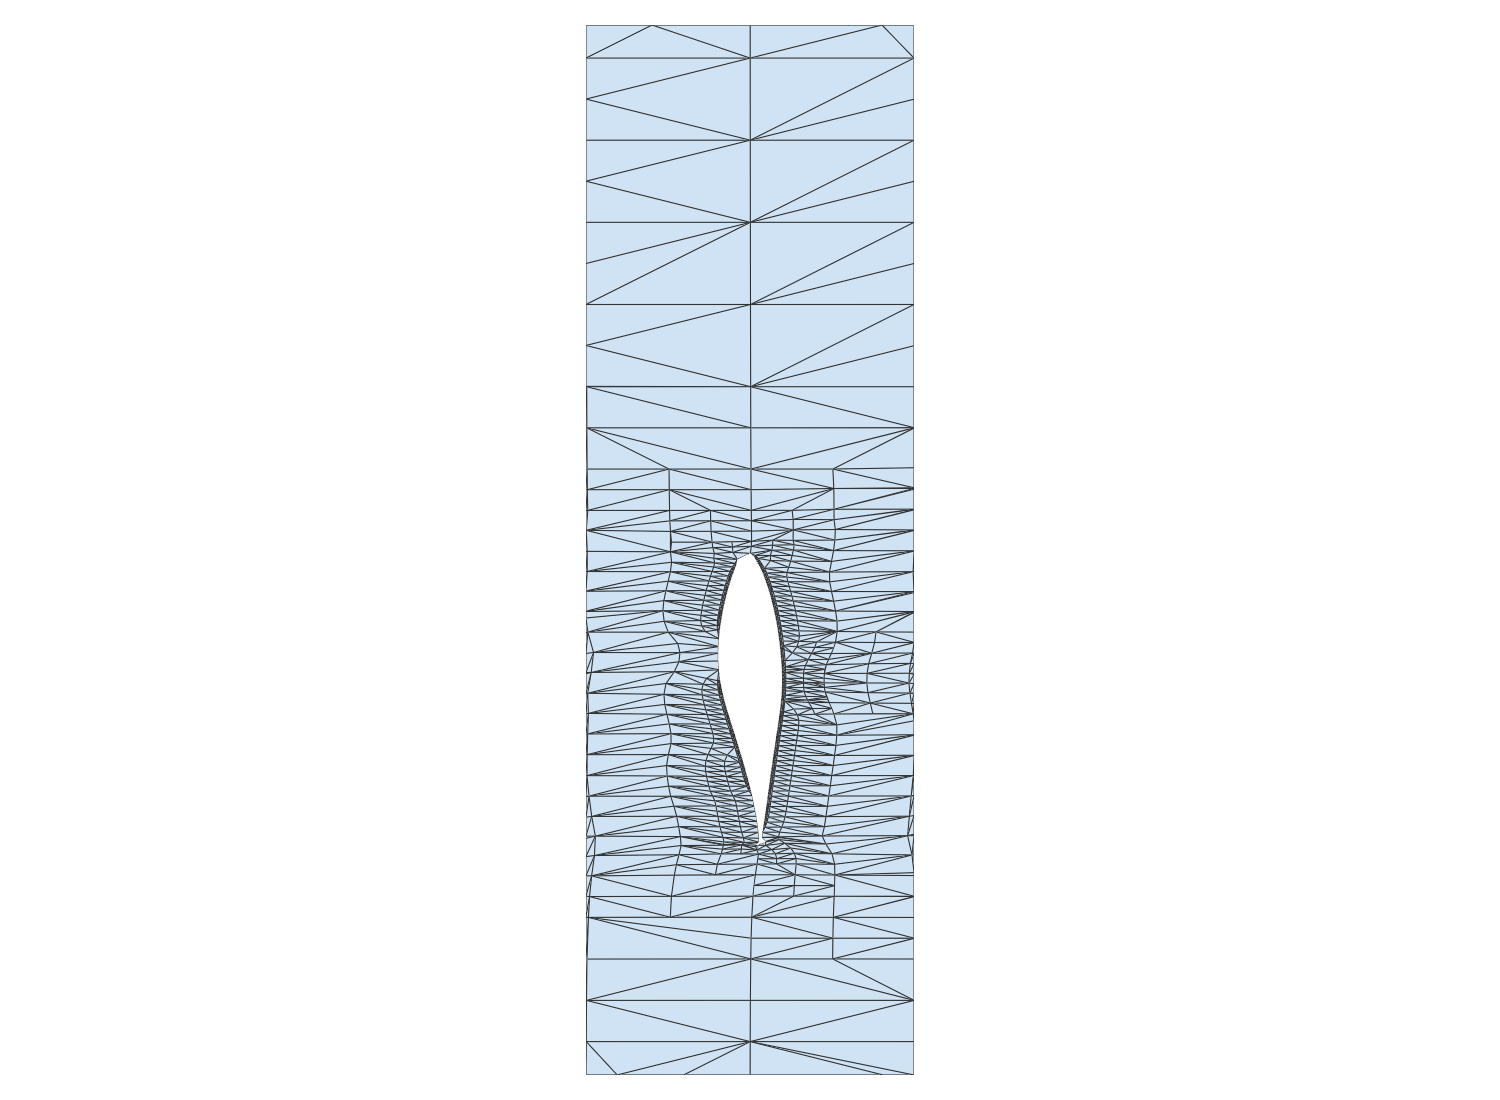
\includegraphics[width=\linewidth,height=0.36\textheight,keepaspectratio]{nrel_mesh_section_zoom.png}\\[1mm]
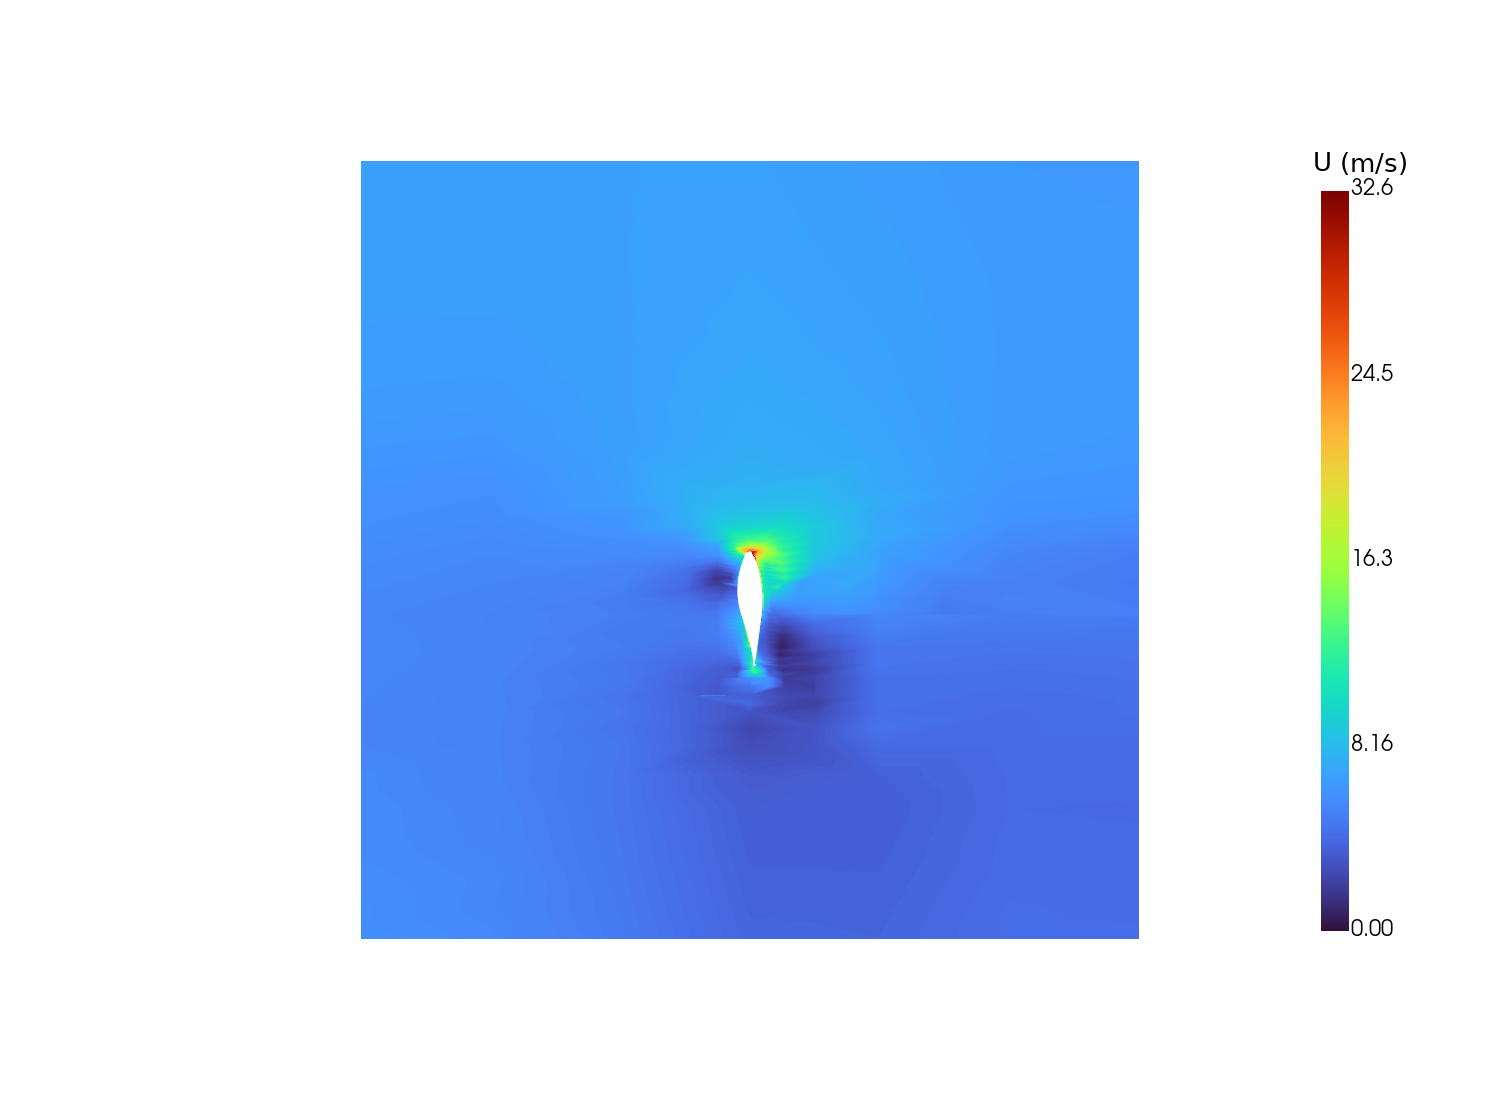
\includegraphics[width=\linewidth,height=0.36\textheight,keepaspectratio]{nrel_U_section.png}
\end{columns}
\end{frame}

\begin{frame}{3. VKI LS89 (highly loaded transonic turbine guide-vane cascade)}
\status{\PART: 7 conditions, all crashed at 63--93\% of target time}{Validation data: \VYES}
\begin{casetab}{\textwidth}
\rw{Geometry}{Linear cascade of the VKI LS89 vane: chord 67.647 mm, pitch 57.5 mm, stagger 55$^\circ$; 2D section}
\rw{Domain and mesh}{One blade passage, periodic; 7-block Plot3D grid converted (Python 3 rewrite of \texttt{p3d2gmsh}), 56,844 hex cells, 16 stitched interfaces, front/back \texttt{empty}}
\rw{Fluid}{Air, perfect gas, \texttt{hePsiThermo}, Sutherland viscosity}
\rw{Physics and solver}{Compressible, transient, density-based \texttt{rhoCentralFoam}; run \textbf{laminar} (SST block present but inactive). \texttt{rhoSimpleFoam} failed on 13 \textmu m trailing-edge cells}
\rw{Rotation model}{None (stationary cascade); \texttt{cyclic} pitchwise periodicity}
\rw{Boundary conditions}{Inlet: total pressure 1.435 MPa (MUR43) and total temperature 420 K; outlet: static pressure 0.904 MPa; blade: no-slip, adiabatic}
\rw{Operating point}{MUR43--MUR49: $P_0$ 1.433--1.608 MPa, $T_0=420$ K, $M_{2,is}$ = 0.84, 0.875, 1.02, Re$_2=10^6$}
\rw{Validation data}{Blade-surface isentropic Mach number and pressure (digitised \texttt{mach.lay}, \texttt{pressure.lay}); heat-transfer data in TN 174}
\rw{References}{Arts, Lambert de Rouvroit, Rutherford (1990) VKI Technical Note 174; AboutFlow benchmark test case 2 (QMUL)}
\rw{Gap / next step}{Restart from checkpoints, fix the floating-point crash in the thermo library, add SST, compare surface Mach}
\end{casetab}
\end{frame}

\begin{frame}{4. NASA Rotor 37 (isolated transonic axial compressor rotor)}
\status{\PART: crashes after $\sim10^{-6}$ s}{Validation data: \VYES}
\begin{casetab}{\textwidth}
\rw{Geometry}{36 MCA blades, tip speed 454 m/s, rig tip clearance 0.356 mm (0.45\% span; case uses 0.35 mm); blade rebuilt from the MERIDL geometry file (own parser)}
\rw{Domain and mesh}{Single passage, 10$^\circ$ periodic; 214--258k cells; 42 skewed faces (max 7.3)}
\rw{Fluid}{Air, perfect gas}
\rw{Physics and solver}{Compressible, \texttt{rhoPimpleFoam}; run \textbf{laminar} (SST block present but inactive), ramped $\omega$}
\rw{Rotation model}{\textbf{MRF}, 17,188.7 rpm (1800 rad/s); periodic sides as \texttt{cyclicAMI} pair}
\rw{Boundary conditions}{Inlet: total pressure 101,325 Pa, total temperature 288.15 K; outlet: static pressure 213,391 Pa (estimated from design PR); hub, shroud, blade: no-slip}
\rw{Operating point}{Design: PR 2.106, adiabatic efficiency 0.889, 20.19 kg/s; speedline from choke to near stall}
\rw{Validation data}{Speedline (PR, efficiency vs mass flow), radial total pressure/temperature and flow angle at stations 1 and 4, laser anemometry; Excel archive \texttt{Rotor37\_exp.zip} downloaded}
\rw{References}{Reid \& Moore (1978) NASA TP-1337; Suder \& Celestina (1996) \emph{J.\ Turbomach.}\ 118(2):218--229; Denton (1997) \emph{J.\ Therm.\ Sci.}\ 6:1--13; Dunham (1998) AGARD-AR-355}
\rw{Gap / next step}{Improve tip and periodic mesh, start at low back-pressure and ramp, turn on SST, then run a speedline}
\end{casetab}
\end{frame}

\begin{frame}{5. Timisoara swirl generator (Politehnica Univ.\ Timisoara)}
\status{\PART: stable to $t=0.238$ s, then SIGFPE}{Validation data: \VDL\ (paper)}
\begin{columns}[T]
\column{.70\textwidth}
\begin{casetab}{\linewidth}
\rw{Geometry}{4 leaned struts $\to$ 13 guide vanes $\to$ free 10-blade runner $\to$ convergent--divergent test section (reproduces the vortex rope of a Francis draft tube at part load)}
\rw{Domain and mesh}{Full 360$^\circ$; shipped mesh 2.70M hex cells, 18 patches; rotating zone 708,050 cells; max non-orth.\ 75$^\circ$ at AMI faces}
\rw{Fluid}{Water, incompressible, $\nu=10^{-6}$ m$^2$/s}
\rw{Physics and solver}{Transient URANS, \texttt{pimpleFoam}, RNG $k$-$\varepsilon$}
\rw{Rotation model}{\textbf{Sliding mesh}: \texttt{dynamicMotionSolverFvMesh} (solid-body rotation), 3 \texttt{cyclicAMI} interfaces; $\omega=96.342$ rad/s (920 rpm). Ported from foam-extend GGI}
\rw{Boundary conditions}{Inlet: axial velocity 1.69765 m/s; outlet: \texttt{fixedMean} $p=0$; runner: \texttt{movingWallVelocity}; other walls: no-slip}
\rw{Operating point}{30 L/s; free runner measured at 920 rpm (design 870 rpm)}
\rw{Validation data}{LDV mean velocity profiles in the cone (used by Petit et al.\ 2011) and unsteady wall pressure (Bosioc et al.\ 2012); not on this machine}
\rw{References}{Susan-Resiga et al.\ (2006) \emph{J.\ Fluids Eng.}\ 128:177--189; Bosioc et al.\ (2012) \emph{J.\ Fluids Eng.}\ 134(8):081104; Petit et al.\ (2011) \emph{IJFMS} 4(1):199--208}
\rw{Gap / next step}{Restart from checkpoint, run several rope periods (1--4 days on 10 cores), average and compare LDV}
\end{casetab}
\column{.28\textwidth}
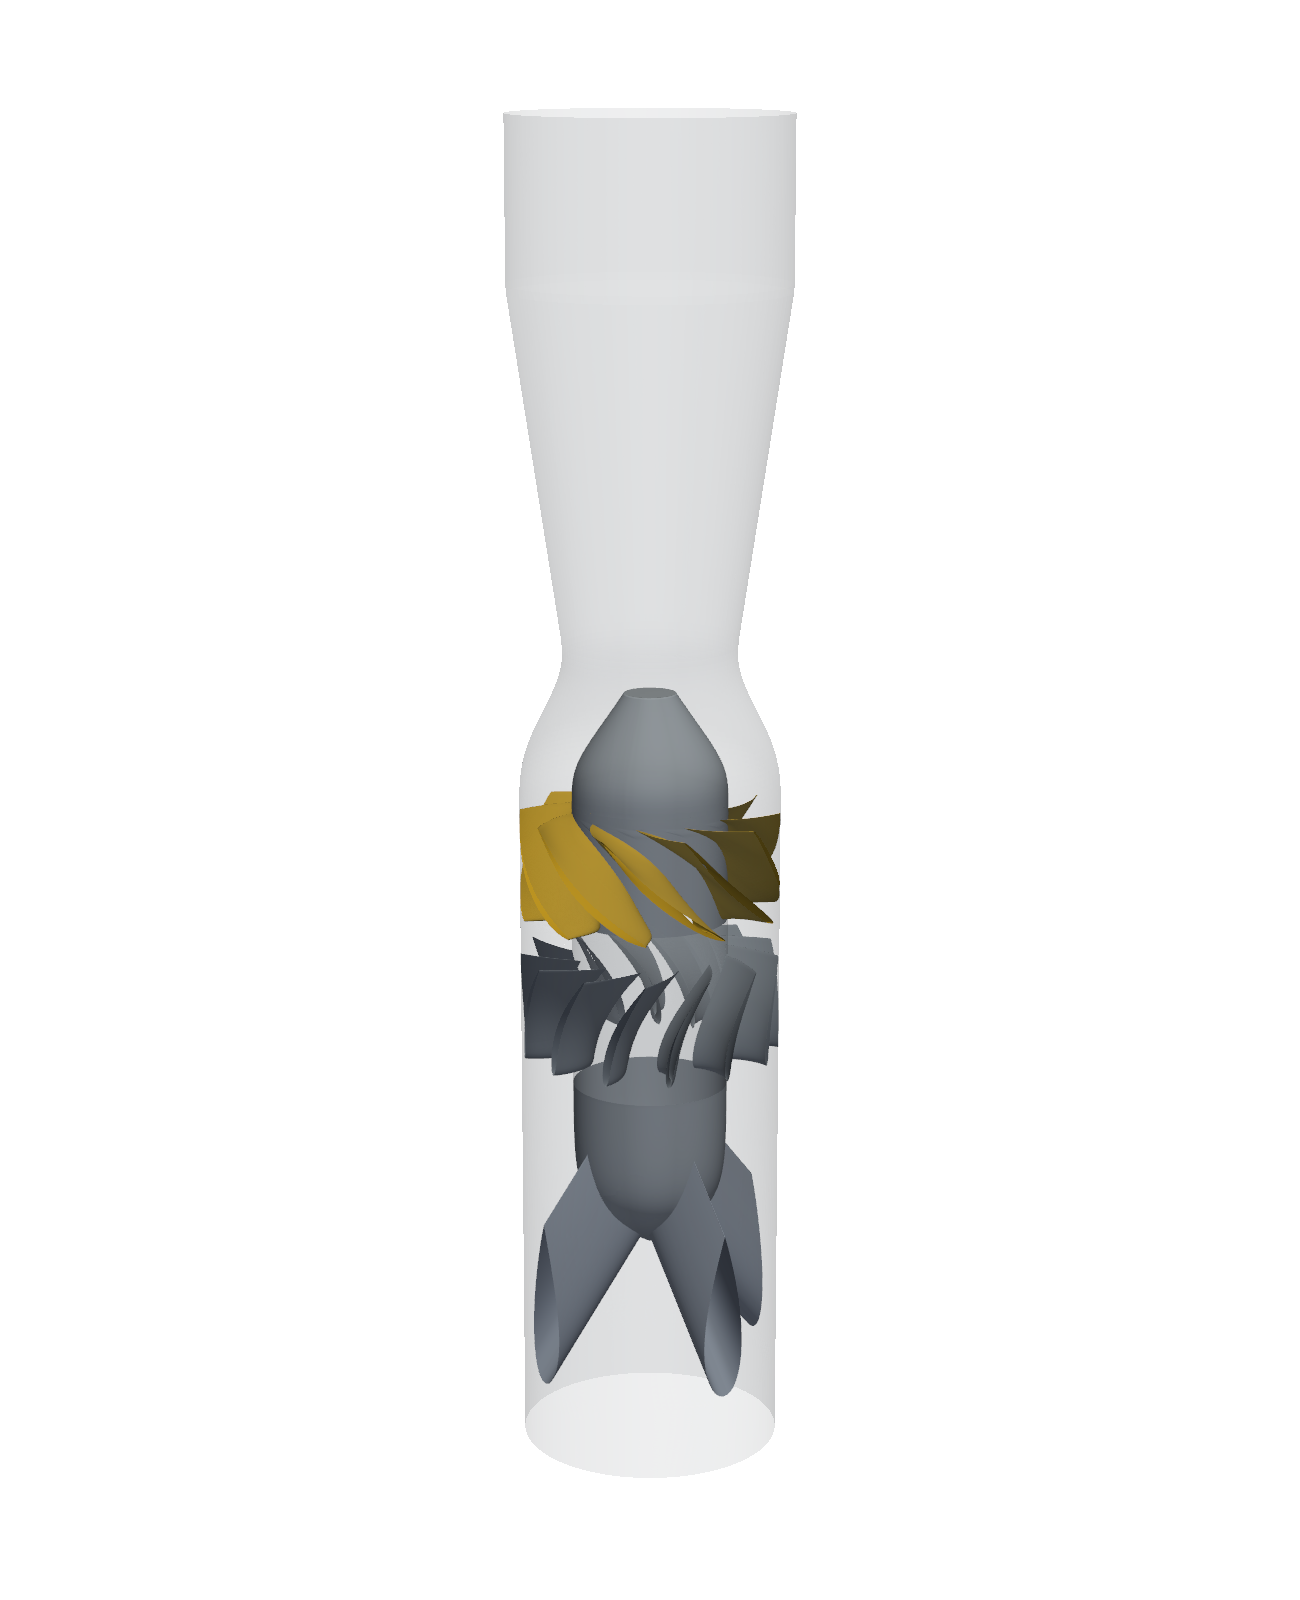
\includegraphics[width=\linewidth,height=0.36\textheight,keepaspectratio]{tim_geometry.png}\\[1mm]

\includegraphics[width=\linewidth,height=0.36\textheight,keepaspectratio]{tim_mesh_ami_zoom.png}
\end{columns}
\end{frame}

\begin{frame}{6. axialTurbine (TurboWG teaching case, 6 rotor--stator methods)}
\status{\RAN: all 6 methods agree within 1.7\% at the runner outlet}{Validation data: \VNO}
\begin{columns}[T]
\column{.70\textwidth}
\begin{casetab}{\linewidth}
\rw{Geometry}{Synthetic axial hydro stage: guide vanes $\to$ 5-blade runner $\to$ draft tube}
\rw{Domain and mesh}{Single passage (cases 1--5) or full 5-blade annulus (case 6); 1,400 / 3,700 / 18,500 cells}
\rw{Fluid}{Incompressible, $\nu=10^{-5}$ m$^2$/s (non-dimensional teaching set-up)}
\rw{Physics and solver}{Steady (\texttt{SRFSimpleFoam}, \texttt{simpleFoam}) and transient (\texttt{SRFPimpleFoam}, \texttt{pimpleFoam}); standard $k$-$\varepsilon$}
\rw{Rotation model}{\textbf{All of them}: SRF steady and transient; MRF + \texttt{cyclicPeriodicAMI}; MRF + \texttt{mixingPlane}; rotating mesh with AMI, 1 blade and 5 blades; $\omega=-10$ rad/s}
\rw{Boundary conditions}{Inlet: axial velocity 1 m/s; outlet: zero-gradient U, fixed $p$; walls: no-slip}
\rw{Operating point}{Single design point}
\rw{Validation data}{No experiment exists for this geometry; method-vs-method comparison only (axial U within 1.7\%, flow angle within 4.3$^\circ$)}
\rw{References}{Nilsson, H., rotating-machinery training, OpenFOAM Workshops OFW7 (2012) and OFW10 (2015); Beaudoin et al.\ (2014) mixingPlane, IOP Conf.\ Ser.}
\rw{Gap / next step}{Cannot be validated; keep as a verification case for the rotation models}
\end{casetab}
\column{.28\textwidth}
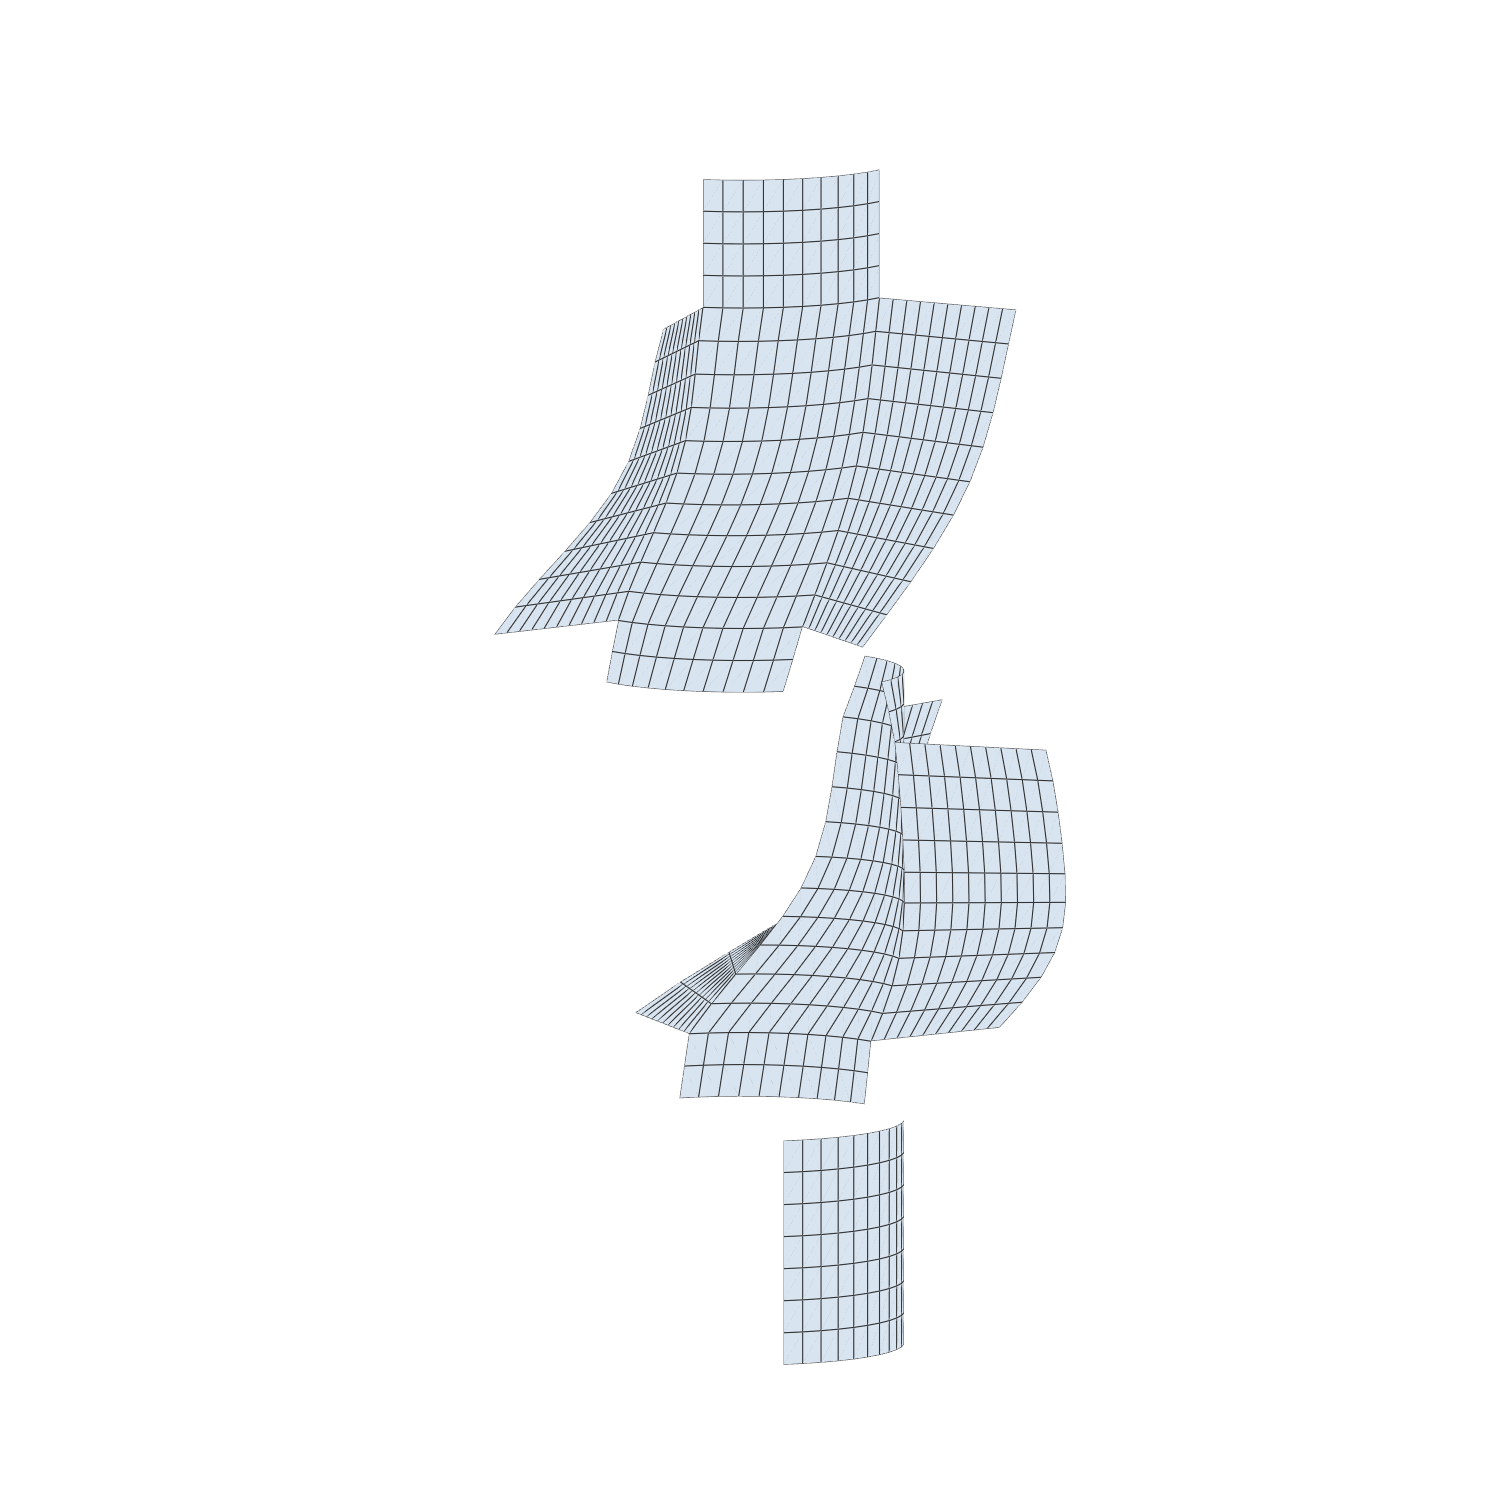
\includegraphics[width=\linewidth,height=0.36\textheight,keepaspectratio]{axial_mesh_blades.png}\\[1mm]
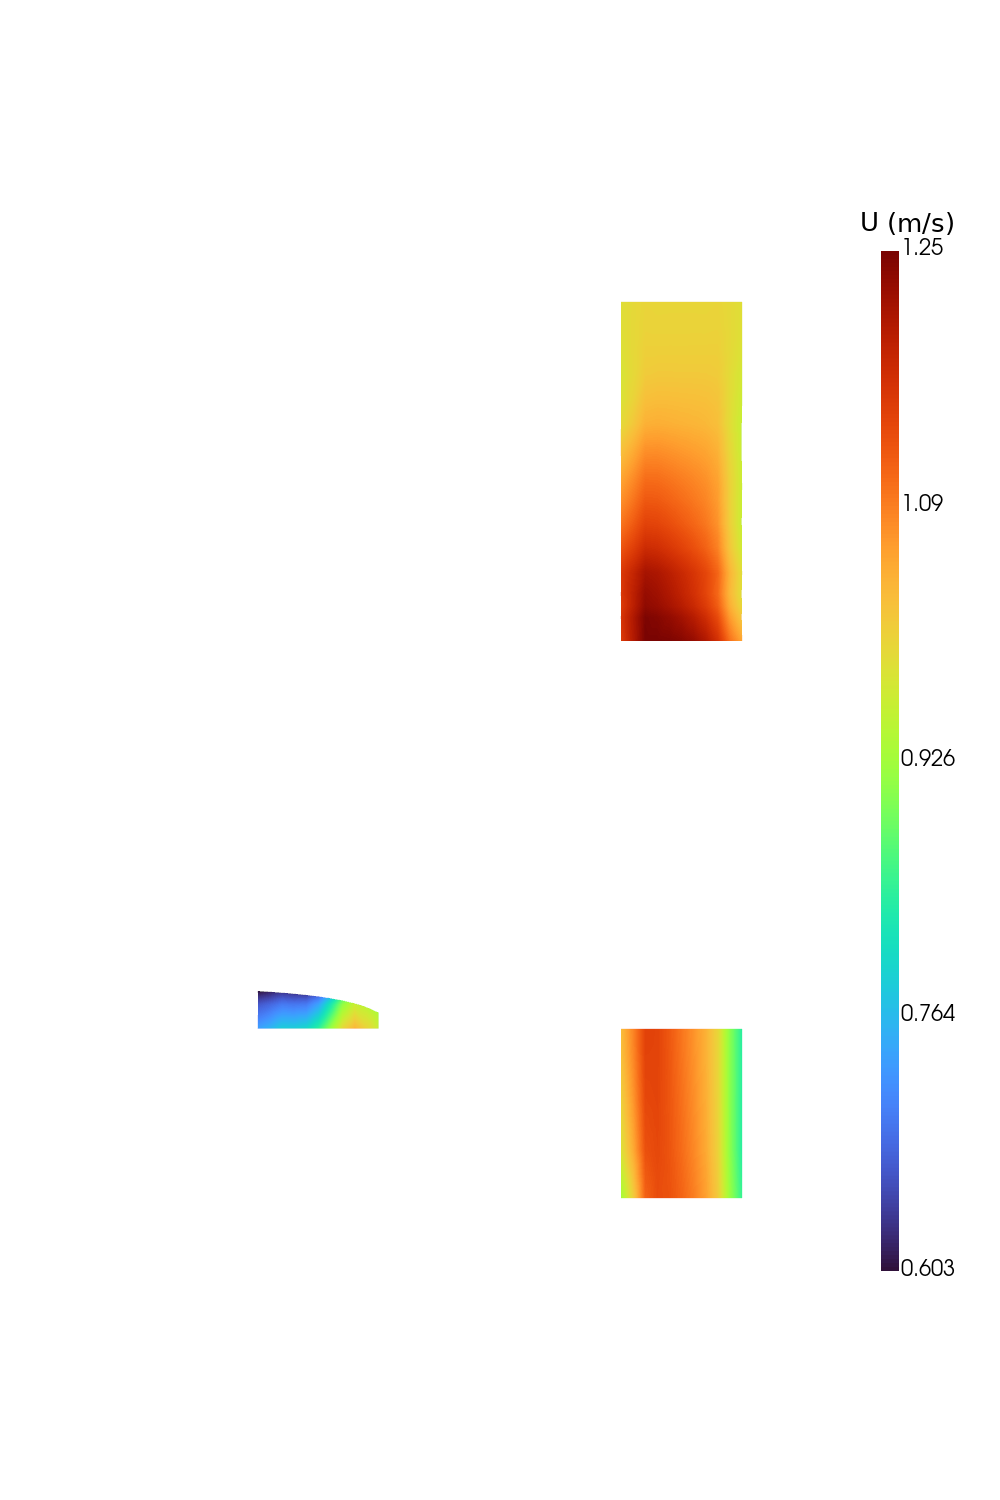
\includegraphics[width=\linewidth,height=0.36\textheight,keepaspectratio]{axial_U.png}
\end{columns}
\end{frame}

%================ B. Setup only
\section{Setup only}

\begin{frame}{7. Turbine-99 (Hölleforsen Kaplan draft tube, Vattenfall)}
\status{\SETUP: dictionaries, no mesh}{Validation data: \VNO\ (raw data offline)}
\begin{casetab}{\textwidth}
\rw{Geometry}{1:11 model of the Hölleforsen sharp-heel elbow draft tube, runner $D=0.5$ m: runner cone, elbow, rectangular diffuser. CAD file not downloadable (host dead since 2010)}
\rw{Domain and mesh}{\emph{Planned}: draft tube only, from the inlet section below the runner to the outlet; hex mesh to be built from the KBwiki geometry description}
\rw{Fluid}{Water, incompressible}
\rw{Physics and solver}{\emph{Planned}: steady RANS, \texttt{simpleFoam}, $k$-$\omega$ SST (skeleton present)}
\rw{Rotation model}{None for the flow; rotating runner-cone wall (595 rpm)}
\rw{Boundary conditions}{\emph{Planned}: inlet = measured LDV axial and tangential mean/RMS profiles at section Ia (radial component missing, to be modelled); outlet: static pressure; cone: rotating wall; walls: no-slip}
\rw{Operating point}{Case T (on-cam, 60\% load): $H=4.5$ m, 595 rpm, $Q$ = 0.522--0.528 m$^3$/s, Re$_D$ $\approx$ 1.75M}
\rw{Validation data}{Wall pressure recovery and LDV velocity at sections Ia, Ib, II, III; only described in ERCOFTAC KBwiki AC6-07, raw files not public}
\rw{References}{Andersson (2000) Turbine 99 workshop proceedings, ISSN 1402-1536; ERCOFTAC KBwiki AC6-07 (Karlsson); Nilsson \& Page (2005), Turbine-99 III, Porjus}
\rw{Gap / next step}{Obtain CAD and inlet/validation data from Vattenfall or Luleå; otherwise not feasible}
\end{casetab}
\end{frame}

\begin{frame}{8. Aachen 1.5-stage axial turbine (RWTH Aachen, IST)}
\status{\SETUP: 3 meshes converted from SU2, not run}{Validation data: \VNO\ (SU2 result only)}
\begin{casetab}{\textwidth}
\rw{Geometry}{Stator 1 $\to$ rotor $\to$ stator 2; modified VKI stator vanes, Traupel rotor profile; untwisted, constant hub/tip; for CFD the stator count is raised from 36 to 41 so every row has 41}
\rw{Domain and mesh}{Single passage per row, 8.78$^\circ$ ($360^\circ/41$) periodic; 3 OpenFOAM meshes converted from the SU2 coarse mesh}
\rw{Fluid}{Air, ideal gas ($\gamma=1.4$, $R=287.058$), Sutherland viscosity}
\rw{Physics and solver}{\emph{Planned}: steady compressible RANS, \texttt{rhoSimpleFoam}, SA or $k$-$\omega$ SST (SU2 used SA + wall functions)}
\rw{Rotation model}{\textbf{MRF} rotor, $\omega=-366.52$ rad/s (3500 rpm); \textbf{mixingPlane} between the 3 rows (compressible + mixingPlane untested in v2412)}
\rw{Boundary conditions}{Inlet: total pressure 158,245 Pa, total temperature 308.26 K, axial; outlet: static pressure 110,051 Pa; TI 2.5\%, $\nu_t/\nu=100$; walls: no-slip}
\rw{Operating point}{Total-to-static PR $\approx$ 1.44, motion Mach 0.35}
\rw{Validation data}{RWTH measurements not public; converged SU2 mixing-plane solution available for code-to-code comparison}
\rw{References}{Gallus, Zeschky \& Hah (1995) \emph{J.\ Turbomach.}\ 117(4):562--570; SU2 Aachen turbine tutorial; Oliani et al.\ (2022), new OpenFOAM turbomachinery solver applied to a 1.5-stage turbine}
\rw{Gap / next step}{Test compressible + mixingPlane; request IST data or accept code-to-code comparison only}
\end{casetab}
\end{frame}

\begin{frame}{9. Pelton turbine (NTNU Waterpower Lab reference design)}
\status{\SETUP: dictionaries, no mesh}{Validation data: efficiency published; CAD on request}
\begin{casetab}{\textwidth}
\rw{Geometry}{Horizontal single-jet Pelton: runner $D=513$ mm (pitch radius 256.7 mm), 23 buckets, bucket width 114.2 mm, jet diameter 35 mm; geometry and data ``available upon request}
\rw{Domain and mesh}{\emph{Planned}: nozzle + jet region (static) and runner sector or full runner (rotating), casing}
\rw{Fluid}{Water and air, two-phase, immiscible, isothermal}
\rw{Physics and solver}{\emph{Planned}: transient VOF, \texttt{interFoam}, $k$-$\omega$ SST}
\rw{Rotation model}{\textbf{Sliding mesh} with \texttt{cyclicACMI} (jet crosses the interface); overset \texttt{overInterDyMFoam} as fallback. MRF not suitable}
\rw{Boundary conditions}{\emph{Planned}: nozzle inlet $\alpha=1$, jet velocity $\sqrt{2gH}\approx37$ m/s; casing outlets atmospheric total pressure; buckets: moving walls; $\omega\approx65$ rad/s (placeholder, not sourced)}
\rw{Operating point}{$H=70$ m, best-efficiency speed to be confirmed}
\rw{Validation data}{Measured efficiency at $H=70$ m (max 77.75\%) and visual inspection (Solemslie \& Dahlhaug 2014); NTUA casing data as a cross-check}
\rw{References}{Solemslie \& Dahlhaug (2012) IOP EES 15:032005, (2014) IOP EES 22:012004; Petley \& Aggidis (2019) \emph{IJFMS} 12(4); Rygg (2013) NTNU MSc thesis, interDyMFoam + AMI}
\rw{Gap / next step}{Request bucket geometry from NTNU; highest compute cost of all cases (several revolutions at VOF Courant limit)}
\end{casetab}
\end{frame}

\begin{frame}{10. Mini-ORC radial-inflow turbine (TU Delft, ORCHID)}
\status{\SETUP: draft dictionaries only}{Validation data: \VNO\ (no measurements yet)}
\begin{casetab}{\textwidth}
\rw{Geometry}{Single-stage radial-inflow turbine, 12 nozzle vanes, rotor $D_2=51.5$ mm, 12 kW; meanline and CFD design published, no 3D blade coordinates}
\rw{Domain and mesh}{\emph{Planned}: one nozzle passage + one rotor passage, periodic}
\rw{Fluid}{Siloxane MM (hexamethyldisiloxane), \textbf{non-ideal (dense) gas}}
\rw{Physics and solver}{\emph{Planned}: compressible RANS with a real-gas equation of state (Peng--Robinson or CoolProp tables); no validated NICFD solver in v2412, needs a new solver family}
\rw{Rotation model}{\textbf{MRF} rotor + mixingPlane (or frozen rotor) at the nozzle--rotor interface; 98,000 rpm}
\rw{Boundary conditions}{\emph{Planned}: inlet total pressure 1810 kPa, total temperature 573 K; outlet static pressure 44.3 kPa}
\rw{Operating point}{Volume ratio 48, nozzle exit angle 78$^\circ$, design $\eta_{ts}$ 83\% (meanline); ORCHID rig limit 25 bar, 300$^\circ$C}
\rw{Validation data}{No published turbine measurements; only the design-method CFD of de Servi et al.}
\rw{References}{de Servi, Burigana, Pini, Colonna (2019) \emph{J.\ Eng.\ Gas Turbines Power} 141(9):091021; Head et al.\ (2016) ORCHID preliminary design}
\rw{Gap / next step}{Not feasible until a real-gas solver is built and measurements are published}
\end{casetab}
\end{frame}

%================ C. Planned, not started
\section{Planned, not started}

\begin{frame}{11. PPTC VP1304 cavitating propeller (SVA Potsdam, SMP'11)}
\status{\PLAN: open water validated; cavitation templates only}{Validation data: \VYES}
\begin{columns}[T]
\column{.70\textwidth}
\begin{casetab}{\linewidth}
\rw{Geometry}{5-blade right-handed CPP VP1304, $D=0.25$ m, $P_{0.7}/D=1.635$, $A_E/A_0=0.779$; cavitation-tunnel hub cap (differs from open-water rig)}
\rw{Domain and mesh}{\emph{Planned}: K15A tunnel section 600$\times$600 mm or open domain; reuse the validated M3 snappyHexMesh set-up (1.16M cells) with tip refinement}
\rw{Fluid}{Water + vapour (Schnerr--Sauer); measured $\rho=997.5$ kg/m$^3$, $\nu=9.4\times10^{-7}$ m$^2$/s, $p_v\approx2.8$ kPa}
\rw{Physics and solver}{\emph{Planned}: \texttt{interPhaseChangeFoam}, VOF + Schnerr--Sauer, $k$-$\omega$ SST}
\rw{Rotation model}{\textbf{MRF} for the first pass; \textbf{sliding mesh} (\texttt{cyclicAMI}) for transient cavity shapes}
\rw{Boundary conditions}{\emph{Planned}: inlet velocity from $J$; outlet pressure set from $\sigma_n$; propeller: rotating no-slip; tunnel walls: slip}
\rw{Operating point}{SVA test cases 2.3.1/2.3.2/2.3.3: $J$ = 1.019 / 1.269 / 1.408, $\sigma_n$ = 2.024 / 1.424 / 2.000, $n=25$ s$^{-1}$}
\rw{Validation data}{Cavity sketches, photos and videos; cavitating $K_T$, $K_Q$; LDV planes (report 3754); all in \texttt{references/}}
\rw{References}{SVA reports 3752, 3753, 3754 (Potsdam, 2011); Gaggero \& Villa (2018) \emph{J.\ Mar.\ Sci.\ Appl.}\ 17(1):1--20}
\rw{Gap / next step}{Strongest new case: geometry, mesh and data are ready}
\end{casetab}
\column{.28\textwidth}
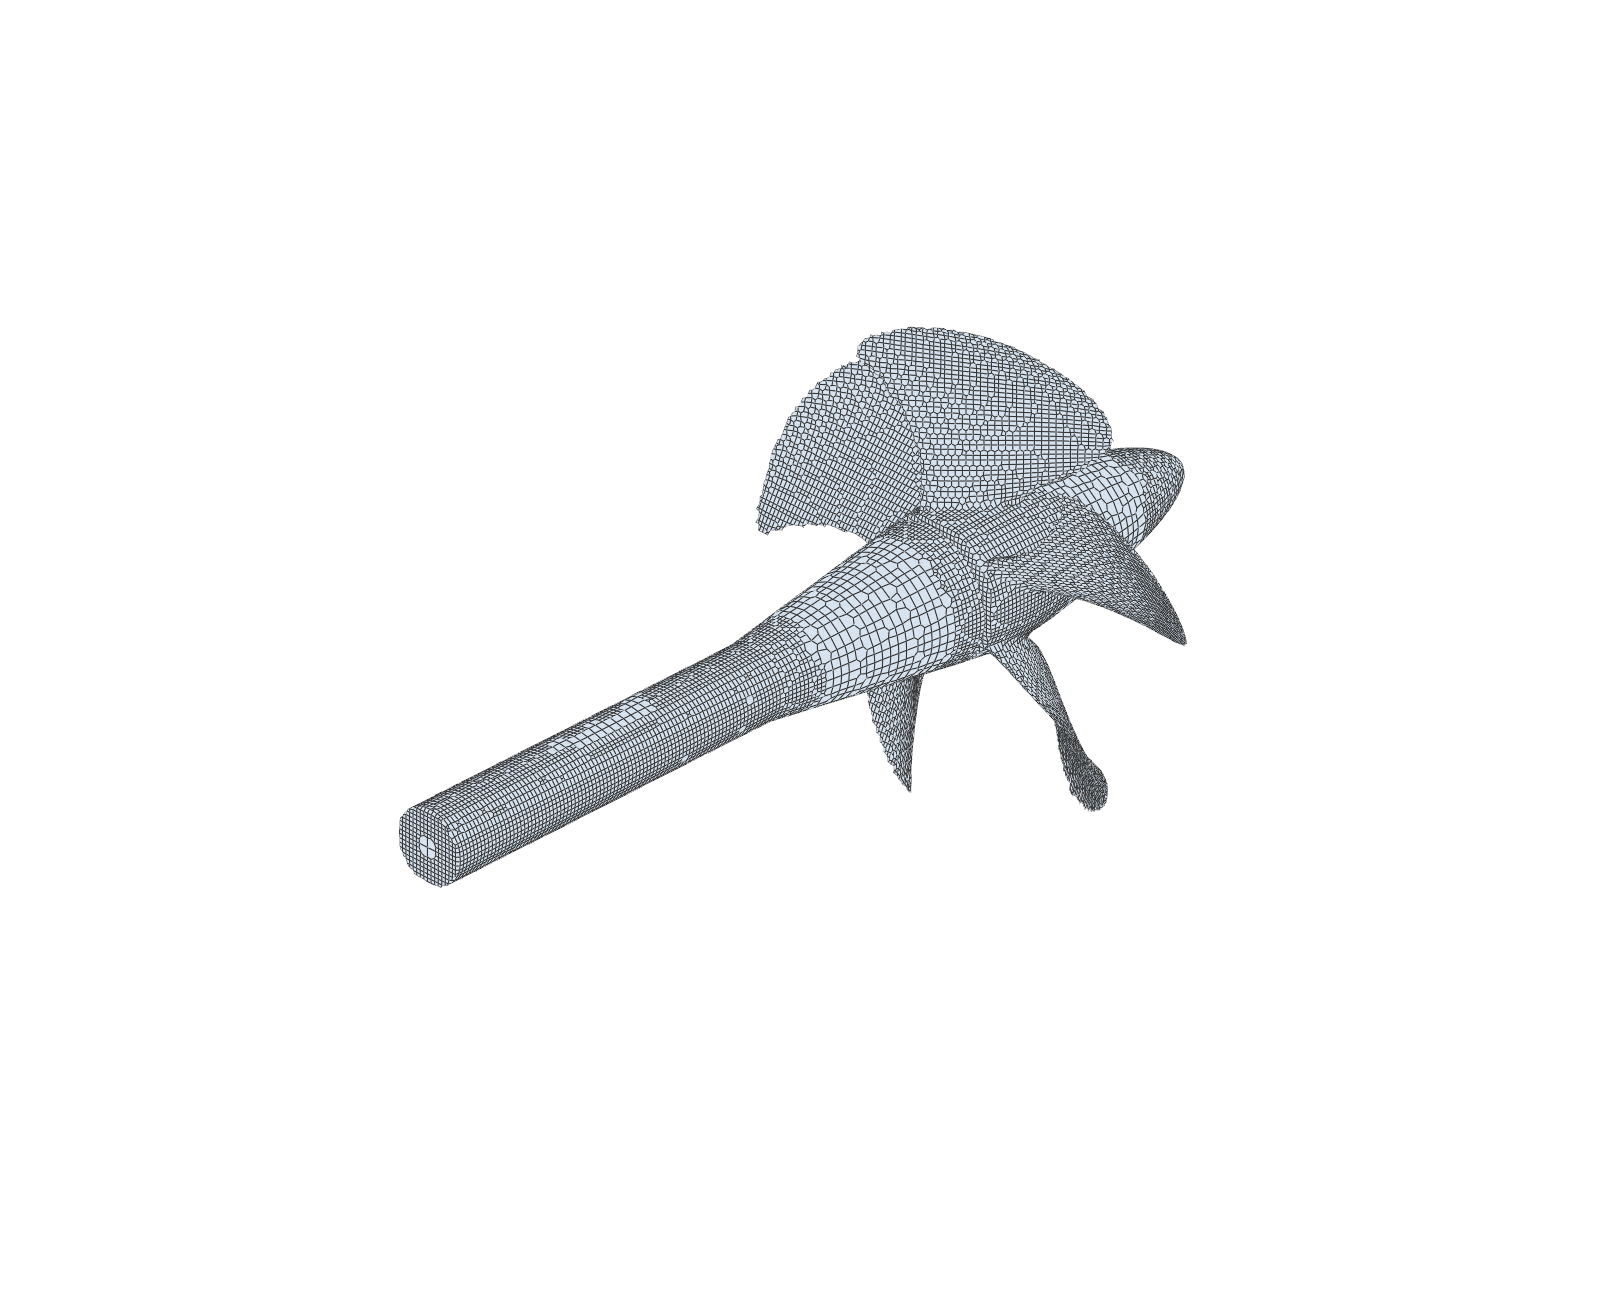
\includegraphics[width=\linewidth,height=0.36\textheight,keepaspectratio]{pptc_mesh_blade.png}\\[1mm]
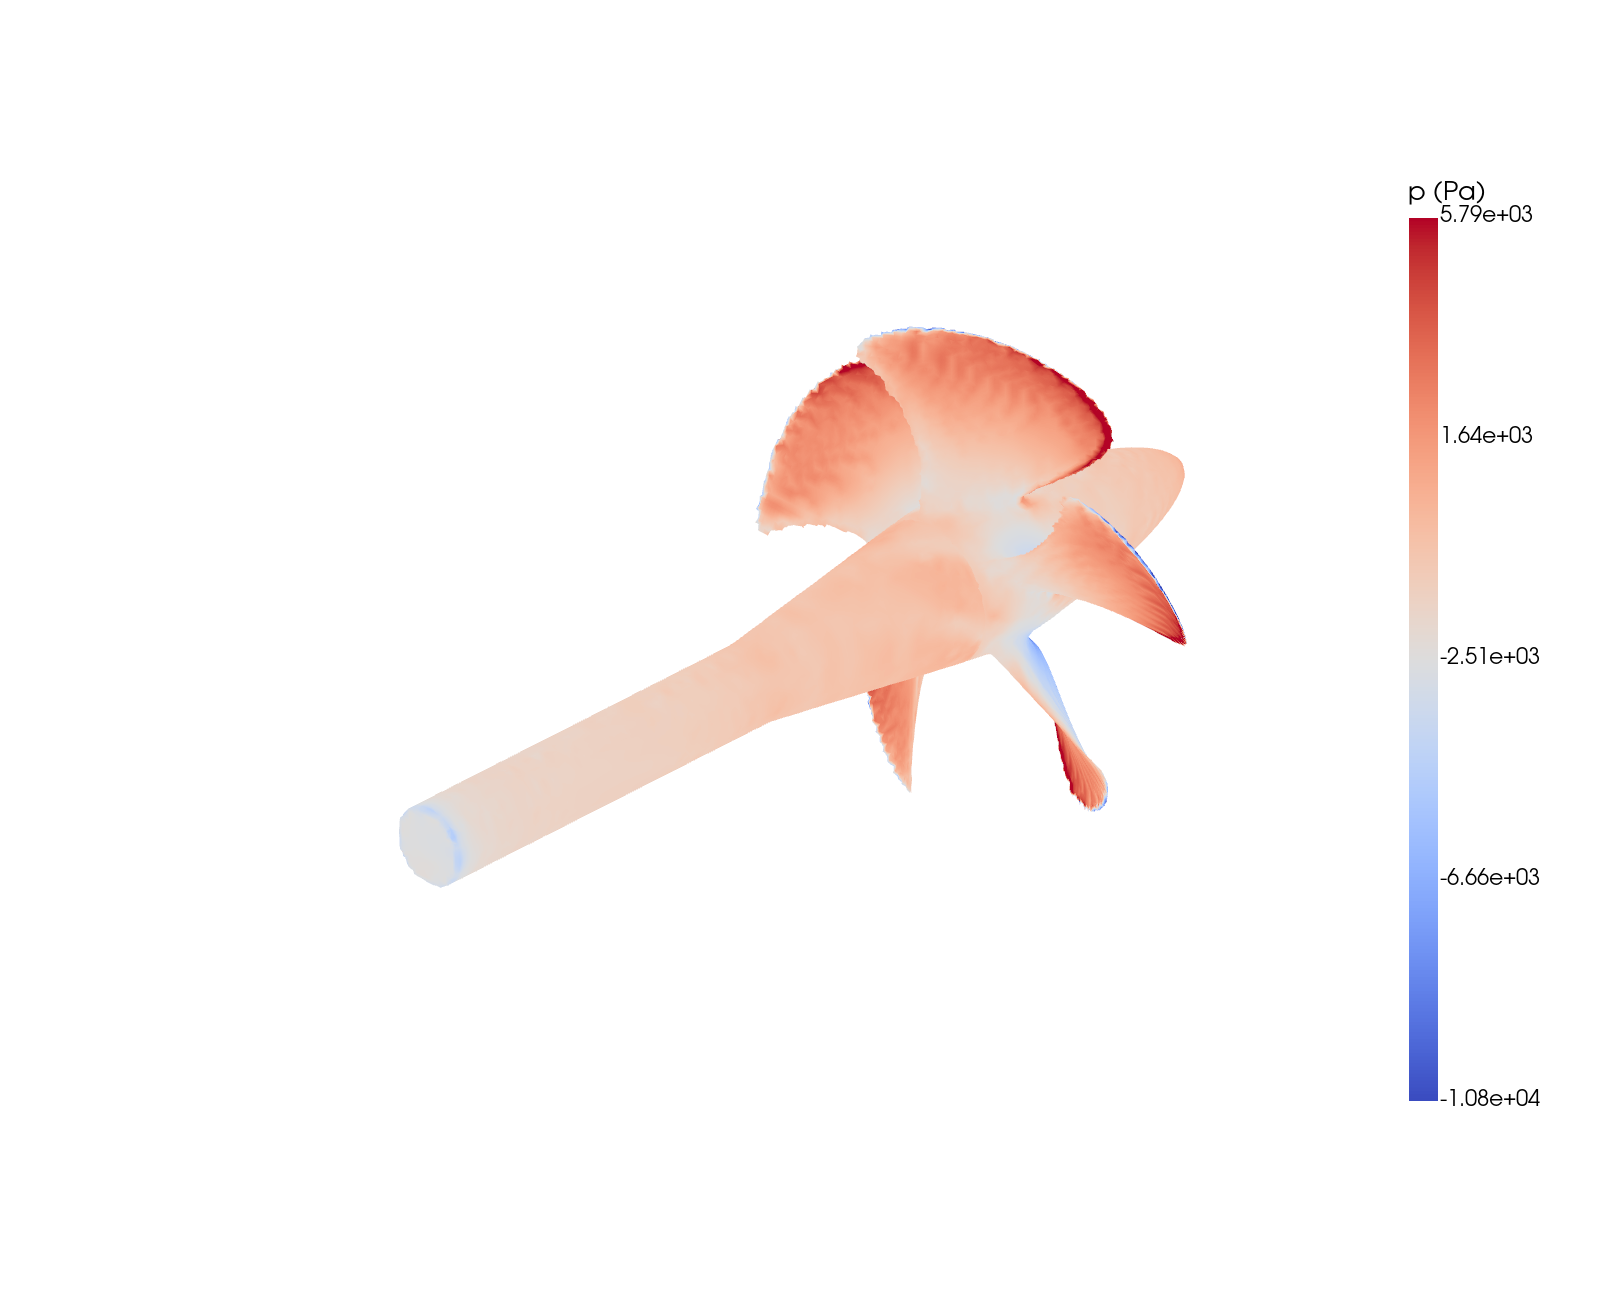
\includegraphics[width=\linewidth,height=0.36\textheight,keepaspectratio]{pptc_p_blade.png}
\end{columns}
\end{frame}

\begin{frame}{12. SHF centrifugal pump impeller (Société Hydrotechnique de France, air model)}
\status{\PLAN: correction, this is \emph{not} the ERCOFTAC U3 rig}{Validation data: published (PIV, wall pressure)}
\begin{casetab}{\textwidth}
\rw{Geometry}{Radial pump impeller, 7 blades, outlet radius 0.2566 m, outlet height 38.5 mm, outlet blade angle 22.5$^\circ$; tested with a vaneless diffuser, vaned diffusers (8 channel-type or 11 cascade-type vanes) and an industrial volute}
\rw{Domain and mesh}{\emph{Planned}: full 360$^\circ$ impeller + diffuser (rotor--stator interaction is not periodic)}
\rw{Fluid}{Air at 25$^\circ$C (low-speed, treated as incompressible)}
\rw{Physics and solver}{\emph{Planned}: steady RANS (\texttt{simpleFoam}), then transient sliding mesh for blade-position-resolved comparison}
\rw{Rotation model}{\textbf{MRF} (frozen rotor at fixed blade position) or \textbf{sliding mesh} (\texttt{cyclicAMI})}
\rw{Boundary conditions}{\emph{Planned}: inlet flow rate; outlet static pressure; walls: no-slip}
\rw{Operating point}{1710 rpm, design flow $Q_n=0.337$ m$^3$/s, tip speed 45.95 m/s; tests at 0.30--1.63 $Q_n$}
\rw{Validation data}{2D PIV of impeller outlet and vaneless diffuser (Wuibaut et al.\ 2001); mean and unsteady wall pressure at 114 taps in one blade passage (Godinho Patricio 1999); directional-probe traverses with vaned diffuser and volute (El Hajem et al.\ 1998)}
\rw{References}{Wuibaut et al.\ (2001) \emph{Proc.\ IMechE A} 215(6); Godinho Patricio (1999) PhD thesis, Univ.\ Lille; El Hajem et al.\ (1998) \emph{La Houille Blanche} 7; Atif, Benmansour, Bois (2010) \emph{Int.\ J.\ Rotating Mach.}\ 706043}
\rw{Gap / next step}{Earlier ``duplicate'' decision was wrong; full blade geometry availability to be confirmed with Arts et Métiers / Lille (LML)}
\end{casetab}
\end{frame}

\begin{frame}{13. NASA Stage 35 (single-stage transonic axial compressor)}
\status{\PLAN: backlog}{Validation data: \VDL}
\begin{casetab}{\textwidth}
\rw{Geometry}{Rotor 35 (36 blades, tip solidity 1.3, aspect ratio 1.19) + stator 35 (46 blades, aspect ratio 1.26); one of four inlet stages (35--38) of NASA TP-1337}
\rw{Domain and mesh}{\emph{Planned}: single passage per row, periodic; structured blade mesh}
\rw{Fluid}{Air, perfect gas}
\rw{Physics and solver}{\emph{Planned}: steady compressible RANS, \texttt{rhoSimpleFoam}, $k$-$\omega$ SST}
\rw{Rotation model}{\textbf{MRF} rotor + \textbf{mixingPlane} to the stator}
\rw{Boundary conditions}{\emph{Planned}: inlet standard total pressure and temperature; outlet static pressure swept along the speedline}
\rw{Operating point}{Design: 17,188.7 rpm, tip speed 455 m/s, 20.19 kg/s, stage PR 1.82, stage adiabatic efficiency 0.828}
\rw{Validation data}{Overall performance maps and radial surveys of total pressure, temperature and flow angle (NASA TP-1337, TP-1338)}
\rw{References}{Reid \& Moore (1978) NASA TP-1337; Reid \& Moore (1978) NASA TP-1338 (blade-element data)}
\rw{Gap / next step}{Do after Rotor 37: same speed, flow and tip speed, so set-up and blade parser carry over}
\end{casetab}
\end{frame}

\begin{frame}{14. Radiver (centrifugal compressor with vaned diffuser, RWTH Aachen / MTU)}
\status{\PLAN: backlog}{Validation data: \VDL\ (open test case)}
\begin{casetab}{\textwidth}
\rw{Geometry}{Semi-open impeller with 15 backward-curved blades (no splitters); wedge vaned diffuser with 23 vanes, adjustable in two degrees of freedom; rig commissioned by MTU, run at RWTH IST}
\rw{Domain and mesh}{\emph{Planned}: one impeller passage + one diffuser passage (non-matching pitch handled by the interface)}
\rw{Fluid}{Air, perfect gas}
\rw{Physics and solver}{\emph{Planned}: steady compressible RANS, \texttt{rhoSimpleFoam}, $k$-$\omega$ SST}
\rw{Rotation model}{\textbf{MRF} impeller + \textbf{mixingPlane} at the impeller--diffuser gap (frozen rotor as a check)}
\rw{Boundary conditions}{\emph{Planned}: inlet total pressure and temperature; outlet static pressure or mass flow}
\rw{Operating point}{Design speed 35,200 rpm, design pressure ratio 4; several diffuser vane settings}
\rw{Validation data}{Steady and unsteady measurements (performance, PIV, unsteady pressure) for several diffuser configurations; geometry and data released to the public domain (RWTH IST open test cases)}
\rw{References}{Ziegler, Gallus \& Niehuis (2003) \emph{J.\ Turbomach.}\ 125(1):173--182 (Part I) and 183--192 (Part II); RWTH IST ``Open Testcases'' page}
\rw{Gap / next step}{Request the open-test-case package from RWTH IST}
\end{casetab}
\end{frame}

\begin{frame}{15. Krain impeller (high-pressure-ratio centrifugal compressor, DLR)}
\status{\PLAN: backlog}{Validation data: published; geometry incomplete}
\begin{casetab}{\textwidth}
\rw{Geometry}{Unshrouded impeller, 24 full blades, 30$^\circ$ backsweep at exit, vaneless diffuser; published geometry does not fully define the blade (reconstruction needed)}
\rw{Domain and mesh}{\emph{Planned}: one blade passage with tip clearance + vaneless diffuser, periodic}
\rw{Fluid}{Air, perfect gas}
\rw{Physics and solver}{\emph{Planned}: steady compressible RANS, \texttt{rhoSimpleFoam}, $k$-$\omega$ SST}
\rw{Rotation model}{\textbf{MRF} impeller (single rotating passage)}
\rw{Boundary conditions}{\emph{Planned}: inlet total pressure and temperature; outlet mass flow or static pressure}
\rw{Operating point}{Design 22,363 rpm, 4.0 kg/s, total rotor pressure ratio 4.7}
\rw{Validation data}{Laser-two-focus (L2F) velocity measurements upstream, along the passage and downstream of the impeller; performance data}
\rw{References}{Krain (1988) ``Swirling impeller flow'', \emph{J.\ Turbomach.}\ 110(1):122--128; Eisenlohr, Krain, Richter, Tiede (2002) ASME GT2002-30394}
\rw{Gap / next step}{Geometry reconstruction risk; lower priority than Radiver and HECC}
\end{casetab}
\end{frame}

\begin{frame}{16. NASA HECC (High-Efficiency Centrifugal Compressor, NASA Glenn CE-18)}
\status{\PLAN: backlog}{Validation data: \VDL\ (public archive)}
\begin{casetab}{\textwidth}
\rw{Geometry}{Impeller with 15 main/splitter blade pairs (backsweep 32--42$^\circ$), exit diameter 17.0 in; vaned diffuser with 20 main/splitter vane pairs; 90$^\circ$ bend; 60 exit guide vanes}
\rw{Domain and mesh}{\emph{Planned}: one impeller, one diffuser and one EGV passage, periodic, tip clearance 0.012 in}
\rw{Fluid}{Air, perfect gas}
\rw{Physics and solver}{\emph{Planned}: steady compressible RANS, \texttt{rhoSimpleFoam}, $k$-$\omega$ SST}
\rw{Rotation model}{\textbf{MRF} impeller + \textbf{mixingPlane} at impeller--diffuser and diffuser--EGV interfaces}
\rw{Boundary conditions}{\emph{Planned}: inlet total pressure 11 psia (rig), total temperature; outlet static pressure swept to the map}
\rw{Operating point}{Design corrected speed 21,789 rpm, $U_2=1615$ ft/s; design-intent PR 4.85 (14.7 psia) / 4.80 (11 psia), measured 4.68; inlet corrected flow 10.85 lbm/s measured; work factor 0.79 design, 0.81 measured}
\rw{Validation data}{Public data archive: stage and subcomponent performance maps, static pressures, 3-hole probe surveys at diffuser exit}
\rw{References}{Braunscheidel, Welch, Skoch, Medic, Sharma (2014) AIAA paper, NTRS 20140016535; Harrison et al.\ (2024) NASA/TM-20240003692/REV1, NTRS 20250000831}
\rw{Gap / next step}{Best open centrifugal-compressor data set; download the archive first}
\end{casetab}
\end{frame}

\begin{frame}{17. NASA SDT fan R4 (Source Diagnostic Test)}
\status{\PLAN: backlog}{Validation data: data public, CAD not}
\begin{casetab}{\textwidth}
\rw{Geometry}{1/5-scale high-bypass fan, 22 in diameter, 22 blades, designed by GE Aircraft Engines; OGV sets: Baseline 54 vanes, Low Count 26 vanes, Low Noise; blade CAD not public}
\rw{Domain and mesh}{\emph{Planned}: one rotor passage + one OGV passage, periodic, with tip clearance}
\rw{Fluid}{Air, perfect gas}
\rw{Physics and solver}{\emph{Planned}: steady compressible RANS, \texttt{rhoSimpleFoam}, $k$-$\omega$ SST}
\rw{Rotation model}{\textbf{MRF} rotor + \textbf{mixingPlane} to the OGV (rotor-alone case: MRF only)}
\rw{Boundary conditions}{\emph{Planned}: inlet total conditions of the 9$\times$15 ft tunnel; bypass outlet static pressure}
\rw{Operating point}{Design corrected speed 12,657 rpm, corrected tip speed 1,215 ft/s, design stage PR 1.47; approach, cutback and takeoff points}
\rw{Validation data}{Rotor-alone and stage performance, LDV flow measurements (NASA Glenn 9$\times$15 ft Low Speed Wind Tunnel)}
\rw{References}{Hughes, Jeracki, Woodward, Miller (2005) NASA/TM-2005-211681 (AIAA-2002-2426); Van Zante et al., SDT LDV report, NTRS 20030066234}
\rw{Gap / next step}{Not feasible without the blade geometry; confirm access with NASA Glenn / GE}
\end{casetab}
\end{frame}

\begin{frame}{18. MEXICO rotor (EU project MEXICO, IEA Wind Task 29 Mexnext)}
\status{\PLAN: backlog}{Validation data: consortium access}
\begin{casetab}{\textwidth}
\rw{Geometry}{3-bladed rotor, $D=4.5$ m, DU91-W2-250, RISØ-A1-21 and NACA 64-418 sections, with nacelle; DNW LLF 9.5$\times$9.5 m open test section}
\rw{Domain and mesh}{\emph{Planned}: full rotor (or 120$^\circ$ periodic) in the open-jet test section}
\rw{Fluid}{Air, incompressible}
\rw{Physics and solver}{\emph{Planned}: steady RANS, \texttt{simpleFoam}, $k$-$\omega$ SST}
\rw{Rotation model}{\textbf{MRF} rotor for axial flow (sliding mesh for yawed cases)}
\rw{Boundary conditions}{\emph{Planned}: inlet uniform velocity; outlet static pressure; open-jet / far-field boundary; blades: no-slip}
\rw{Operating point}{Axial flow, 424.5 rpm, pitch $-2.3^\circ$, $U_\infty$ = 10, 15, 24 m/s (tip speed ratio 10, 6.7, 4.2)}
\rw{Validation data}{148 Kulite pressure sensors at 25, 35, 60, 82, 92\% radius; rotor loads; PIV wake data}
\rw{References}{Schepers \& Snel (2007) ECN-E--07-042 (MEXICO final report); Schepers, Boorsma, Munduate (2014) \emph{J.\ Phys.\ Conf.\ Ser.}\ 555:012089}
\rw{Gap / next step}{Confirm data access with IEA Wind Task 29/47}
\end{casetab}
\end{frame}

\begin{frame}{19. Wells turbine / oscillating water column (wave energy)}
\status{\PLAN: backlog}{Validation data: depends on chosen rig}
\begin{casetab}{\textwidth}
\rw{Geometry}{Self-rectifying axial air turbine with symmetric (typically NACA 00xx) blades set in the plane of rotation, above an OWC chamber; no single canonical open rig}
\rw{Domain and mesh}{\emph{Planned}: turbine passage (periodic); optional OWC chamber with wave flume}
\rw{Fluid}{Air (turbine); water + air for the chamber}
\rw{Physics and solver}{\emph{Planned}: turbine: transient incompressible RANS, \texttt{pimpleFoam}, $k$-$\omega$ SST, oscillating inflow; chamber: VOF (\texttt{interFoam})}
\rw{Rotation model}{\textbf{MRF} for quasi-steady characteristic curves; \textbf{sliding mesh} for the oscillating cycle}
\rw{Boundary conditions}{\emph{Planned}: inlet time-varying (sinusoidal) velocity or pressure; outlet static pressure; blades: no-slip}
\rw{Operating point}{Flow-coefficient sweep at constant speed (rig-specific)}
\rw{Validation data}{Torque and pressure-drop coefficients vs flow coefficient from the chosen rig (see reviews)}
\rw{References}{Raghunathan (1995) \emph{Prog.\ Aerosp.\ Sci.}\ 31(4):335--386; Shehata et al.\ (2017) \emph{Int.\ J.\ Energy Res.}\ 41:6--38; 16 kW Wells/OWC design for Ecuador (2025) \emph{Processes} 13:2349 (waves in OpenFOAM)}
\rw{Gap / next step}{Choose a rig with open geometry and measurements first}
\end{casetab}
\end{frame}

\begin{frame}{Summary: which cases can be validated}
\small
\begin{columns}[T]
\column{.33\textwidth}
\textbf{\textcolor{ok}{Data in hand or open}}
\begin{itemize}
\item Francis-99 (part load)
\item PPTC cavitating
\item VKI LS89
\item NREL Phase VI
\item NASA Rotor 37
\item Stage 35, HECC, Radiver
\end{itemize}
\column{.33\textwidth}
\textbf{\textcolor{part}{Possible, with cost or access}}
\begin{itemize}
\item Timisoara (1--4 days compute)
\item SHF impeller (geometry access)
\item Aachen (code-to-code only)
\item MEXICO (consortium data)
\item Krain (geometry rebuild)
\item Wells (choose rig)
\end{itemize}
\column{.33\textwidth}
\textbf{\textcolor{bad}{Blocked}}
\begin{itemize}
\item axialTurbine (no experiment)
\item Turbine-99 (CAD, data offline)
\item Pelton (geometry on request)
\item Mini-ORC (no solver, no data)
\item SDT R4 (CAD proprietary)
\end{itemize}
\end{columns}
\end{frame}

\begin{frame}[allowframebreaks]{References (checked 5 October 2026)}
\fontsize{6.6}{7.8}\selectfont
\begin{enumerate}\setlength{\itemsep}{0.5pt}
\item Trivedi C., Cervantes M.J., Gandhi B.K., Dahlhaug O.G. (2013). Experimental and numerical studies for a high head Francis turbine at several operating points. \emph{J.\ Fluids Eng.}\ 135(11):111102. doi:10.1115/1.4024805
\item NTNU Waterpower Lab. Francis-99 2nd workshop data (14--15 Dec 2016), files \texttt{f99w2-exp-*}; www.ntnu.no/wiki/display/vkl/Second+workshop
\item Hand M.M.\ et al.\ (2001). Unsteady Aerodynamics Experiment Phase VI: Wind tunnel test configurations and available data campaigns. NREL/TP-500-29955.
\item Simms D., Schreck S., Hand M., Fingersh L.J. (2001). NREL Unsteady Aerodynamics Experiment in the NASA-Ames wind tunnel: a comparison of predictions to measurements. NREL/TP-500-29494.
\item Arts T., Lambert de Rouvroit M., Rutherford A.W. (1990). Aero-thermal investigation of a highly loaded transonic linear turbine guide vane cascade. VKI Technical Note 174.
\item AboutFlow (QMUL). Test Case 2: VKI LS89. www.aboutflow.sems.qmul.ac.uk/events/munich2016/benchmark/testcase2/
\item Reid L., Moore R.D. (1978). Design and overall performance of four highly loaded, high speed inlet stages for an advanced high-pressure-ratio core compressor. NASA TP-1337.
\item Suder K.L., Celestina M.L. (1996). Experimental and computational investigation of the tip clearance flow in a transonic axial compressor rotor. \emph{J.\ Turbomach.}\ 118(2):218--229.
\item Denton J.D. (1997). Lessons from rotor 37. \emph{J.\ Therm.\ Sci.}\ 6:1--13. doi:10.1007/s11630-997-0010-9
\item Dunham J.\ (ed.) (1998). CFD validation for propulsion system components. AGARD-AR-355.
\item Susan-Resiga R., Ciocan G.D., Anton I., Avellan F. (2006). Analysis of the swirling flow downstream a Francis turbine runner. \emph{J.\ Fluids Eng.}\ 128:177--189.
\item Bosioc A.I., Susan-Resiga R., Muntean S., Tanasa C. (2012). Unsteady pressure analysis of a swirling flow with vortex rope and axial water injection in a discharge cone. \emph{J.\ Fluids Eng.}\ 134(8):081104.
\item Petit O., Bosioc A.I., Nilsson H., Muntean S., Susan-Resiga R.F. (2011). Unsteady simulations of the flow in a swirl generator, using OpenFOAM. \emph{Int.\ J.\ Fluid Mach.\ Syst.}\ 4(1):199--208.
\item Nilsson H. Rotating machinery training (SRF, MRF, moving mesh, coupling interfaces). 7th (2012) and 10th (2015) OpenFOAM Workshops.
\item Andersson U.\ (2000). Turbine 99 -- experiments on draft tube flow (test case T). Proc.\ Turbine 99 Workshop, ISSN 1402-1536.
\item ERCOFTAC Knowledge Base Wiki. Application Challenge AC6-07: Draft tube (contributor R.\ Karlsson, Vattenfall Utveckling AB).
\item Nilsson H., Page M.\ (2005). OpenFOAM simulation of the flow in the Hölleforsen draft tube model. Turbine-99 III, Porjus, 8--9 Dec 2005.
\item Gallus H.E., Zeschky J., Hah C.\ (1995). Endwall and unsteady flow phenomena in an axial turbine stage. \emph{J.\ Turbomach.}\ 117(4):562--570. doi:10.1115/1.2836568
\item SU2. Aachen turbine stage with mixing plane (tutorial). su2code.github.io/tutorials/Aachen\_Turbine/
\item Oliani S.\ et al.\ (2022). A new solver for turbomachinery simulations in OpenFOAM: development and application to a 1.5 axial turbine stage. Conference paper, Univ.\ Ferrara.
\item Solemslie B.W., Dahlhaug O.G.\ (2012). A reference Pelton turbine design. \emph{IOP Conf.\ Ser.: Earth Environ.\ Sci.}\ 15:032005.
\item Solemslie B.W., Dahlhaug O.G.\ (2014). A reference Pelton turbine -- design and efficiency measurements. \emph{IOP Conf.\ Ser.: Earth Environ.\ Sci.}\ 22:012004.
\item Petley S., Aggidis G.A.\ (2019). Estimating the energy loss in Pelton turbine casings by transient CFD and experimental analysis. \emph{Int.\ J.\ Fluid Mach.\ Syst.}\ 12(4).
\item Rygg J.R.\ (2013). CFD analysis of a Pelton turbine in OpenFOAM. MSc thesis, NTNU.
\item de Servi C.M., Burigana M., Pini M., Colonna P.\ (2019). Design method and performance prediction for radial-inflow turbines of high-temperature mini-organic Rankine cycle power systems. \emph{J.\ Eng.\ Gas Turbines Power} 141(9):091021.
\item Head A.J., De Servi C., Casati E., Pini M., Colonna P.\ (2016). Preliminary design of the ORCHID: a facility for studying non-ideal compressible fluid dynamics and testing ORC expanders. ASME Turbo Expo.
\item SVA Potsdam (2011). PPTC open water tests (report 3752); cavitation tests (report 3753); LDV velocity measurements (report 3754).
\item Gaggero S., Villa D.\ (2018). Cavitating propeller performance in inclined shaft conditions with OpenFOAM: PPTC 2015 test case. \emph{J.\ Mar.\ Sci.\ Appl.}\ 17(1):1--20. doi:10.1007/s11804-018-0008-6
\item Wuibaut G., Bois G., Caignaert G., Dupont P., Stanislas M.\ (2001). Analysis of flow velocities within the impeller and the vaneless diffuser of a radial flow pump. \emph{Proc.\ IMechE A} 215(6).
\item Godinho Patricio O.\ (1999). Experimental analysis of the mean and fluctuating pressures inside a single inter-blade passage of a centrifugal pump impeller. PhD thesis, Univ.\ Lille.
\item El Hajem M., Morel R., Spettel F., Bois G.\ (1998). Étude de l'écoulement moyen en sortie de roue d'une pompe centrifuge (roue SHF). \emph{La Houille Blanche} 7.
\item Atif A., Benmansour S., Bois G.\ (2010). Numerical investigation of velocity flow field inside an impeller air model of a centrifugal pump with vaned diffuser interactions and comparison with PIV measurements. \emph{Int.\ J.\ Rotating Mach.}\ 2010:706043; and Atif et al., CFM 2017, Lille (rig data table).
\item Reid L., Moore R.D.\ (1978). Stage 35 single-stage performance and blade-element data (companion to TP-1337). NASA TP-1338.
\item Ziegler K.U., Gallus H.E., Niehuis R.\ (2003). A study on impeller--diffuser interaction, Parts I and II. \emph{J.\ Turbomach.}\ 125(1):173--182, 183--192.
\item RWTH Aachen IST. Open Testcases: Radiver. www.ist.rwth-aachen.de
\item Krain H.\ (1988). Swirling impeller flow. \emph{J.\ Turbomach.}\ 110(1):122--128.
\item Eisenlohr G., Krain H., Richter F.-A., Tiede V.\ (2002). Investigations of the flow through a high pressure ratio centrifugal impeller. ASME GT2002-30394.
\item Braunscheidel E.P., Welch G.E., Skoch G.J., Medic G., Sharma O.P.\ (2014). Aerodynamic performance of a compact, high work-factor centrifugal compressor at the stage and subcomponent level. NTRS 20140016535.
\item Harrison et al.\ (2024). User's guide for the NASA High Efficiency Centrifugal Compressor data archive. NASA/TM-20240003692/REV1, NTRS 20250000831.
\item Hughes C.E., Jeracki R.J., Woodward R.P., Miller C.J.\ (2005). Fan Noise Source Diagnostic Test -- rotor alone aerodynamic performance results. NASA/TM-2005-211681.
\item Schepers J.G., Snel H.\ (2007). Model experiments in controlled conditions (MEXICO), final report. ECN-E--07-042.
\item Schepers J.G., Boorsma K., Munduate X.\ (2014). Final results from Mexnext-I. \emph{J.\ Phys.\ Conf.\ Ser.}\ 555:012089.
\item Raghunathan S.\ (1995). The Wells air turbine for wave energy conversion. \emph{Prog.\ Aerosp.\ Sci.}\ 31(4):335--386.
\item Shehata A.S., Xiao Q., Saqr K.M., Alexander D.\ (2017). Wells turbine for wave energy conversion: a review. \emph{Int.\ J.\ Energy Res.}\ 41:6--38. doi:10.1002/er.3583
\item A dynamic analysis of oscillating water column systems: design of a 16 kW Wells turbine for coastal energy generation in Ecuador (2025). \emph{Processes} 13:2349. doi:10.3390/pr13082349
\end{enumerate}
\end{frame}
\end{document}
